\documentclass[11pt]{article}

% =================================================================
% PREAMBLE
% =================================================================
\usepackage{amsmath, amssymb, amsthm} % For math symbols and environments
\usepackage{graphicx}                % For including images
\usepackage[a4paper, margin=1in]{geometry} % For page layout
\usepackage{tikz}                    % For drawing vector graphics
\usepackage{xcolor}                  % For colors
\usepackage{hyperref}                % For hyperlinks, etc.
\usepackage{fancyvrb}                % For code blocks

% --- TikZ Style Definitions ---
\tikzstyle{axis} = [->, thick]
\tikzstyle{func} = [thick]
\tikzstyle{guide} = [dashed, gray]

% --- Math Macros ---
\newcommand{\R}{\mathbb{R}}
\newcommand{\w}{\mathbf{w}}
\newcommand{\x}{\mathbf{x}}
\newcommand{\y}{\mathbf{y}}
\newcommand{\T}{^T}
\newcommand{\relu}{\text{ReLU}}

% --- Document Info ---
\title{Lecture 2: The Power of Non-Linearity}
\author{From Linear Boundaries to Exponential Expressivity}
\date{}

% =================================================================
% DOCUMENT START
% =================================================================
\begin{document}

\maketitle

\section{From Linear Models to a Single Neuron}

In our last lecture, we revisited linear regression, a model defined by the simple equation $f(\x) = \w\T\x + b$. While fundamental, this model is severely limited; it can only ever learn linear relationships. More critically, stacking multiple linear layers just results in another linear transformation:
\[ \w_2\T(\w_1\T\x + \mathbf{b}_1) + \mathbf{b}_2 = (\w_2\T\w_1\T)\x + (\w_2\T\mathbf{b}_1 + \mathbf{b}_2) = \w_{\text{new}}\T\x + \mathbf{b}_{\text{new}} \]
To learn the complex, non-linear patterns found in the real world, we need our ``magic ingredient": \textbf{non-linearity}. We introduce this by creating an \textbf{artificial neuron}.

\paragraph{The Biological Inspiration (The Threshold)}
The concept of an artificial neuron is inspired by biology. A biological neuron in the brain receives signals from many other neurons. It ``fires"—sending its own signal forward—only when the cumulative input stimulus it receives crosses a certain threshold. Early models like the Perceptron were built on this explicit thresholding idea. The neuron computes a weighted sum of its inputs, and if that sum is greater than a threshold, it outputs 1 (``fires"); otherwise, it outputs 0 (``silent").

\paragraph{The Modern Choice (ReLU) and the Gradient Problem}
Today, the most common activation function is the \textbf{Rectified Linear Unit}, or \textbf{ReLU}, which provides a simple and computationally efficient analogue of this firing threshold.
\begin{equation}
    \relu(z) = \max(0, z) \label{eq:relu}
\end{equation}
The function of a single ReLU neuron is $f(\x) = \relu(\w\T\x + b)$. Here, the term $\w\T\x+b$ represents the total weighted input stimulus. If this stimulus is negative (below the threshold of 0), the neuron is silent (output=0). If the stimulus is positive, the neuron ``fires'' with an intensity proportional to the stimulus.

A key question arises: the ReLU function has a sharp ``corner'' at $z=0$, where its derivative is mathematically undefined. How can we use gradient-based learning? In practice, this is not a problem. The derivative is 0 for all $z<0$ and 1 for all $z>0$. At the single point $z=0$, we can simply assign a value for the gradient; common practice in libraries like PyTorch is to use 0. Since the probability of hitting the exact value $z=0$ during training with floating-point numbers is virtually zero, this mathematical discontinuity has no effect on our ability to train the network.

\section{The Power of a Single Neuron: Creating Boundaries}
Let's build our intuition with the simplest case: a single input $x$. A single ReLU neuron computes $y = \max(0, wx+b)$, transforming a simple line into a ``hinge'' function.

\begin{figure}[h!]
\centering
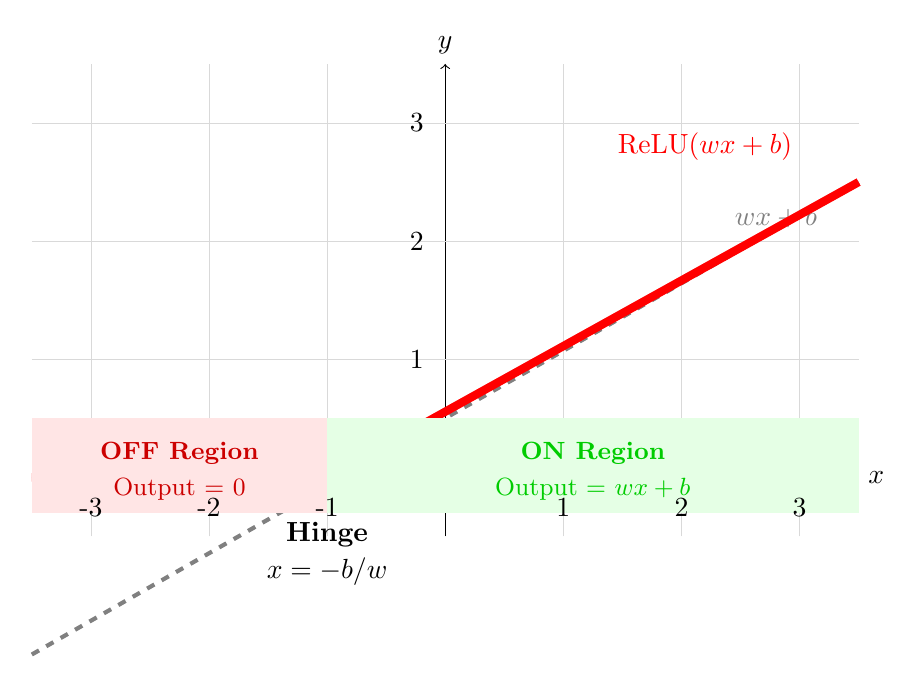
\begin{tikzpicture}[scale=1.5]
    % Axes
    \draw[->] (-3.5,0) -- (3.5,0) node[right] {$x$};
    \draw[->] (0,-0.5) -- (0,3.5) node[above] {$y$};
    
    % Grid for better readability
    \foreach \x in {-3,-2,-1,1,2,3} {
        \draw[very thin, gray!30] (\x, -0.5) -- (\x, 3.5);
    }
    \foreach \y in {1,2,3} {
        \draw[very thin, gray!30] (-3.5, \y) -- (3.5, \y);
    }
    
    % The linear part wx+b (dashed)
    \draw[dashed, gray, line width=1.5pt] (-3.5, -1.5) -- (3.5, 2.5);
    \node[gray] at (2.8, 2.2) {$wx+b$};

    % The ReLU output (thick red)
    \draw[red, line width=3pt] (-3.5,0) -- (-1,0) -- (3.5, 2.5);
    \node[red] at (2.2, 2.8) {$\relu(wx+b)$};

    % Hinge point - very prominent
    \fill[black] (-1,0) circle (4pt);
    \node[below] at (-1,-0.3) {\textbf{Hinge}};
    \node[below] at (-1,-0.6) {$x = -b/w$};
    
    % Region annotations with background
    \fill[red!10] (-3.5,-0.3) rectangle (-1,0.5);
    \fill[green!10] (-1,-0.3) rectangle (3.5,0.5);
    \node[red!80!black, font=\small\bfseries] at (-2.25, 0.2) {\textbf{OFF Region}};
    \node[red!80!black, font=\small] at (-2.25, -0.1) {Output = 0};
    \node[green!80!black, font=\small\bfseries] at (1.25, 0.2) {\textbf{ON Region}};
    \node[green!80!black, font=\small] at (1.25, -0.1) {Output = $wx+b$};
    
    % Axis labels
    \foreach \x in {-3,-2,-1,1,2,3} {
        \node[below] at (\x, -0.1) {\x};
    }
    \foreach \y in {1,2,3} {
        \node[left] at (-0.1, \y) {\y};
    }
\end{tikzpicture}
\caption{Enhanced view of a ReLU neuron: The neuron creates a sharp boundary at $x = -b/w$, dividing the input into ``off'' and ``on'' regions. This is the fundamental building block of neural network expressivity.}
\label{fig:relu_hinge}
\end{figure}

\textbf{Key insight}: The neuron creates a \emph{boundary} in input space. Everything on one side of the boundary gives zero output; everything on the other side gives a linear ramp. This boundary is the fundamental unit of computation.

\section{The Geometric Revolution: From 1D to Higher Dimensions}
The real power becomes apparent in higher dimensions. For a single ReLU neuron with two inputs, $(x_1, x_2)$, the activation boundary is the line $w_1x_1 + w_2x_2 + b = 0$. This line divides the 2D input space into two regions: an ``off'' region and an ``on'' region.

\begin{figure}[h!]
\centering
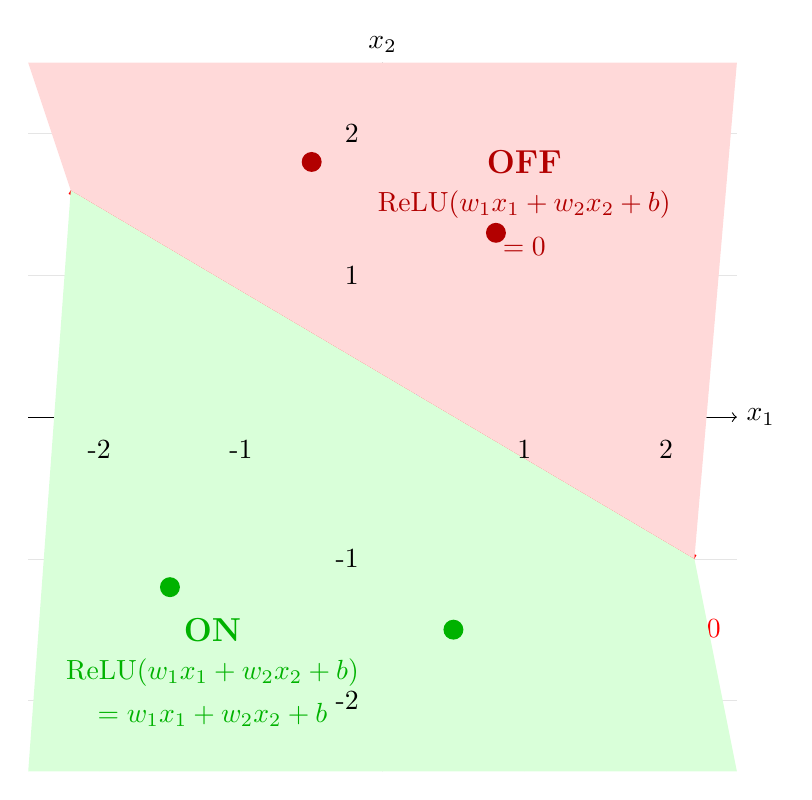
\begin{tikzpicture}[scale=1.8]
    % Set up coordinate system
    \draw[->] (-2.5,0) -- (2.5,0) node[right] {$x_1$};
    \draw[->] (0,-2.5) -- (0,2.5) node[above] {$x_2$};
    
    % Grid
    \foreach \x in {-2,-1,1,2} {
        \draw[very thin, gray!20] (\x, -2.5) -- (\x, 2.5);
    }
    \foreach \y in {-2,-1,1,2} {
        \draw[very thin, gray!20] (-2.5, \y) -- (2.5, \y);
    }
    
    % Decision boundary line
    \draw[red, line width=3pt] (-2.2, 1.6) -- (2.2, -1.0);
    \node[red] at (1.5, -1.5) {$w_1x_1 + w_2x_2 + b = 0$};
    
    % Weight vector (normal to boundary)
    \draw[blue, very thick, ->] (0,0) -- (1.3, 0.85);
    \node[blue] at (1.5, 1.1) {\textbf{w}};
    \node[blue] at (1.5, 0.8) {(normal)};
    
    % Region shading
    \fill[green!15] (-2.5,-2.5) -- (-2.2, 1.6) -- (2.2, -1.0) -- (2.5, -2.5) -- cycle;
    \fill[red!15] (-2.5, 2.5) -- (-2.2, 1.6) -- (2.2, -1.0) -- (2.5, 2.5) -- cycle;
    
    % Region labels
    \node[green!70!black, font=\large\bfseries] at (-1.2, -1.5) {ON};
    \node[green!70!black] at (-1.2, -1.8) {$\relu(w_1x_1 + w_2x_2 + b)$};
    \node[green!70!black] at (-1.2, -2.1) {$= w_1x_1 + w_2x_2 + b$};
    
    \node[red!70!black, font=\large\bfseries] at (1.0, 1.8) {OFF};
    \node[red!70!black] at (1.0, 1.5) {$\relu(w_1x_1 + w_2x_2 + b)$};
    \node[red!70!black] at (1.0, 1.2) {$= 0$};
    
    % Sample points
    \fill[green!70!black] (-1.5, -1.2) circle (2pt);
    \fill[green!70!black] (0.5, -1.5) circle (2pt);
    \fill[red!70!black] (0.8, 1.3) circle (2pt);
    \fill[red!70!black] (-0.5, 1.8) circle (2pt);
    
    % Axis labels
    \foreach \x in {-2,-1,1,2} {
        \node[below] at (\x, -0.1) {\x};
    }
    \foreach \y in {-2,-1,1,2} {
        \node[left] at (-0.1, \y) {\y};
    }
\end{tikzpicture}
\caption{A single ReLU neuron in 2D creates a linear decision boundary. The weight vector \textbf{w} points perpendicular to this boundary. Sample points show how different regions produce different outputs.}
\label{fig:single_neuron_2d}
\end{figure}

\section{The Magic of Multiple Neurons: Exponential Complexity}
When we have a layer of multiple ReLU neurons, each neuron creates its own linear boundary. Together they partition the input space into multiple regions.

\subsection{The Polytope Partitioning}
With $k$ neurons in a layer, we get $k$ different lines (in 2D) that intersect to create a complex partition of space. Each resulting region is a \textbf{convex polytope}—a shape bounded by straight lines. Within each polytope, the entire network layer computes a different linear function.

\begin{figure}[h!]
\centering
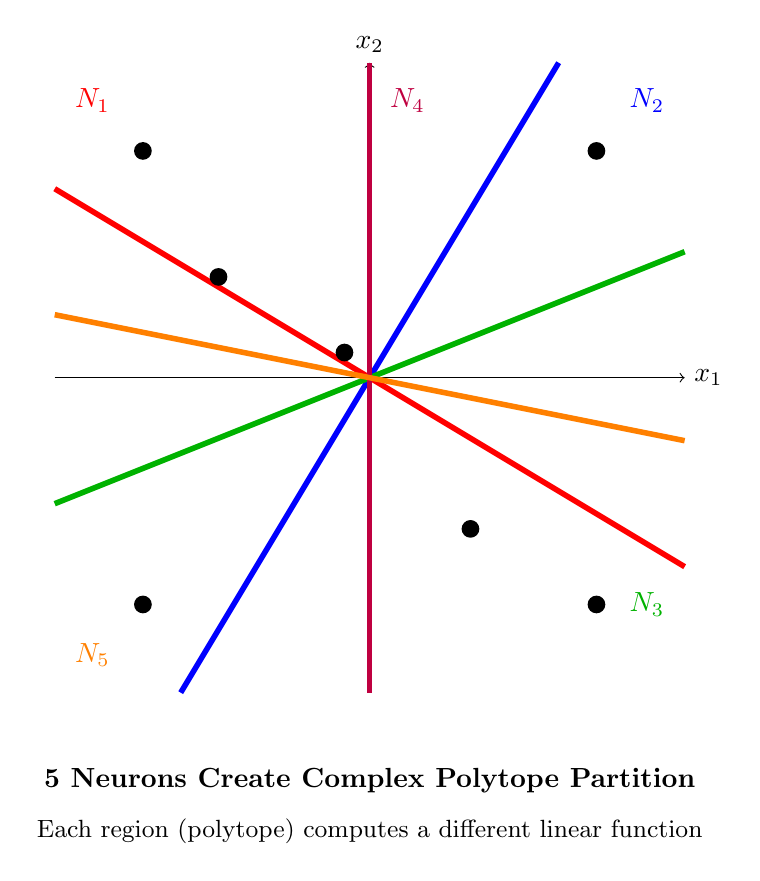
\begin{tikzpicture}[scale=1.6]
    % Coordinate system
    \draw[->] (-2.5,0) -- (2.5,0) node[right] {$x_1$};
    \draw[->] (0,-2.5) -- (0,2.5) node[above] {$x_2$};
    
    % Multiple neuron boundaries with different colors
    \draw[red, line width=2pt] (-2.5, 1.5) -- (2.5, -1.5);
    \draw[blue, line width=2pt] (-1.5, -2.5) -- (1.5, 2.5);
    \draw[green!70!black, line width=2pt] (-2.5, -1) -- (2.5, 1);
    \draw[purple, line width=2pt] (0, -2.5) -- (0, 2.5);
    \draw[orange, line width=2pt] (-2.5, 0.5) -- (2.5, -0.5);
    
    % Label the boundaries
    \node[red] at (-2.2, 2.2) {$N_1$};
    \node[blue] at (2.2, 2.2) {$N_2$};
    \node[green!70!black] at (2.2, -1.8) {$N_3$};
    \node[purple] at (0.3, 2.2) {$N_4$};
    \node[orange] at (-2.2, -2.2) {$N_5$};
    
    % Add sample points in different regions
    \foreach \x/\y in {-1.8/1.8, -1.8/-1.8, 1.8/1.8, 1.8/-1.8, -0.2/0.2, 0.8/-1.2, -1.2/0.8} {
        \fill[black] (\x, \y) circle (2pt);
    }
    
    \node at (0, -3.2) {\textbf{5 Neurons Create Complex Polytope Partition}};
    \node[font=\small] at (0, -3.6) {Each region (polytope) computes a different linear function};
\end{tikzpicture}
\caption{Multiple ReLU neurons create intersecting boundaries that partition the space into convex polytopes. Each black dot represents a point in a different region where the network computes a unique linear function.}
\label{fig:multiple_neurons}
\end{figure}

The number of possible linear regions grows rapidly with the number of neurons. With $k$ neurons in a layer and $d$-dimensional input, you can create up to $O(k^d)$ regions.

\subsection{Combining Neurons: Emergence of Complexity in 1D}
Returning to our 1D example, we can see how combining the outputs of hinge functions created by a hidden layer allows us to construct more complex functions. With just two neurons, we can create a ``bump".

\begin{figure}[h!]
\centering
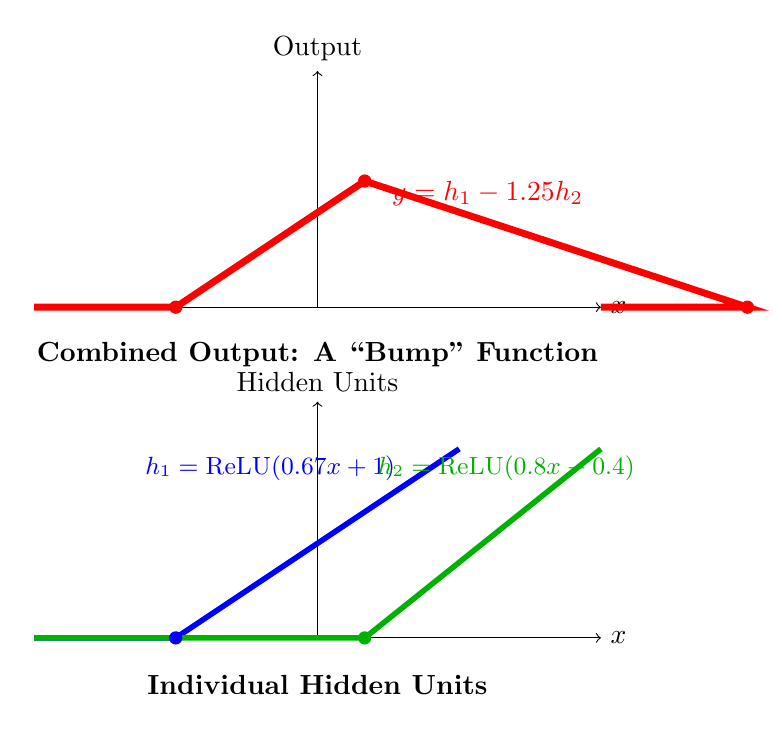
\begin{tikzpicture}[scale=1.2]
    % Bottom plot: Individual Neurons
    \begin{scope}[yshift=-2cm]
        \draw[->] (-3,0) -- (3,0) node[right] {$x$};
        \draw[->] (0,0) -- (0,2.5) node[above] {Hidden Units};
        
        % First neuron (blue hinge)
        \draw[blue, line width=2pt] (-3,0) -- (-1.5,0) -- (1.5, 2);
        \node[blue, font=\small] at (-0.5, 1.8) {$h_1 = \relu(0.67x + 1)$};
        
        % Second neuron (green hinge)
        \draw[green!70!black, line width=2pt] (-3,0) -- (0.5,0) -- (3, 2);
        \node[green!70!black, font=\small] at (2, 1.8) {$h_2 = \relu(0.8x - 0.4)$};
        
        % Mark the hinge points
        \fill[blue] (-1.5,0) circle (2pt);
        \fill[green!70!black] (0.5,0) circle (2pt);
        
        \node at (0, -0.5) {\textbf{Individual Hidden Units}};
    \end{scope}

    % Top plot: Combined Output
    \begin{scope}[yshift=1.5cm]
        \draw[->] (-3,0) -- (3,0) node[right] {$x$};
        \draw[->] (0,0) -- (0,2.5) node[above] {Output};
        
        % Combined output: precise bump calculation
        % h1 = max(0, 0.67x + 1) = max(0, 0.67(x + 1.5))
        % h2 = max(0, 0.8x - 0.4) = max(0, 0.8(x - 0.5))
        % y = h1 - 1.25*h2
        % Breakpoints: x = -1.5 (h1 turns on), x = 0.5 (h2 turns on)
        % At x = 0.5: h1 = 1.335, h2 = 0, so y = 1.335
        % For x > 0.5: y = (0.67x + 1) - 1.25(0.8x - 0.4) = 0.67x + 1 - x + 0.5 = -0.33x + 1.5
        % At x = 1.5/0.33 = 4.55, y = 0
        \draw[red, line width=2.5pt] (-3,0) -- (-1.5,0) -- (0.5,1.335) -- (4.55,0) -- (3,0);
        \node[red] at (1.8, 1.2) {$y = h_1 - 1.25h_2$};
        
        % Mark key points
        \fill[red] (-1.5,0) circle (2pt);
        \fill[red] (0.5,1.335) circle (2pt);
        \fill[red] (4.55,0) circle (2pt);
        
        \node at (0, -0.5) {\textbf{Combined Output: A ``Bump'' Function}};
    \end{scope}
\end{tikzpicture}
\caption{By combining two ReLU neurons with opposite signs in the output layer, we create a ``bump'' function. This demonstrates how linear pieces can be assembled into complex, non-linear shapes.}
\label{fig:bump}
\end{figure}

\section{The Universal Approximation Theorem}
This simple idea—creating bumps—is the intuitive basis for the \textbf{Universal Approximation Theorem}. It states that a neural network with just one hidden layer can, in principle, approximate any continuous function to any desired degree of accuracy.

\textbf{The intuition}: If we can create one ``bump", we can create many bumps of different sizes and positions. By adding thousands of tiny bumps, we can essentially ``paint'' or tile any continuous function we want, like a digital artist using brush strokes. While this theorem is reassuring, it doesn't tell us how to find the right weights—that's the job of our learning algorithm. But it proves that neural networks have the raw expressive power to be universal function approximators.

\section{The Deep Revolution: Why Depth Creates Exponential Power}
The universal approximation theorem tells us that even shallow networks are powerful. So why do we use deep networks? The answer lies in \emph{efficiency} and the geometric structure they create.

\subsection{Bending Boundaries: The Deep Network Advantage}
When we add a second hidden layer, its inputs are the piecewise-linear outputs of the first layer. This means the activation boundaries created by the second layer are no longer straight lines—they can ``bend'' at the boundaries created by the first layer.

\begin{figure}[h!]
\centering
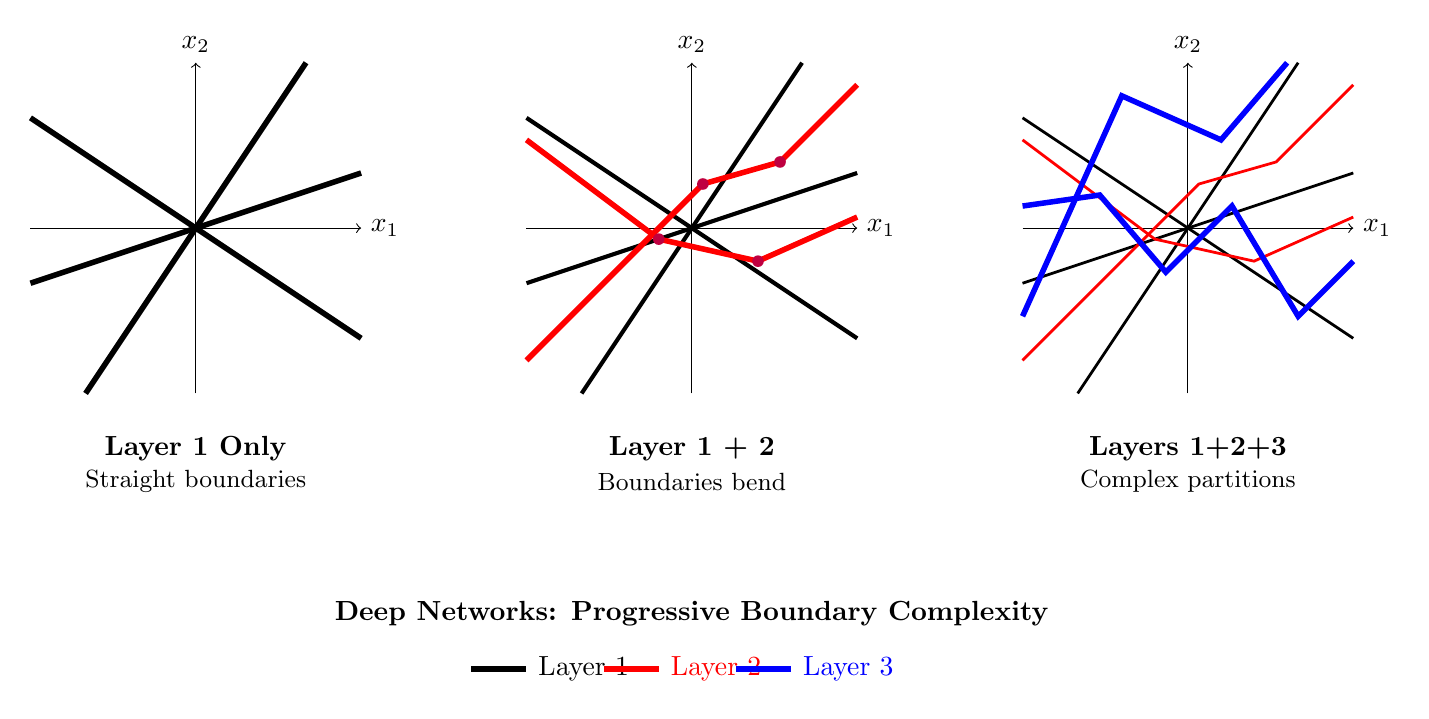
\begin{tikzpicture}[scale=1.4]
    % Layer 1 only
    \begin{scope}[xshift=-4.5cm]
        \draw[->] (-1.5,0) -- (1.5,0) node[right] {$x_1$};
        \draw[->] (0,-1.5) -- (0,1.5) node[above] {$x_2$};
        
        % Layer 1 boundaries (straight)
        \draw[black, line width=2pt] (-1.5, 1) -- (1.5, -1);
        \draw[black, line width=2pt] (-1, -1.5) -- (1, 1.5);
        \draw[black, line width=2pt] (-1.5, -0.5) -- (1.5, 0.5);
        
        \node at (0, -2) {\textbf{Layer 1 Only}};
        \node[font=\small] at (0, -2.3) {Straight boundaries};
    \end{scope}
    
    % Layer 1 + 2
    \begin{scope}[xshift=0cm]
        \draw[->] (-1.5,0) -- (1.5,0) node[right] {$x_1$};
        \draw[->] (0,-1.5) -- (0,1.5) node[above] {$x_2$};
        
        % Layer 1 boundaries
        \draw[black, line width=1.5pt] (-1.5, 1) -- (1.5, -1);
        \draw[black, line width=1.5pt] (-1, -1.5) -- (1, 1.5);
        \draw[black, line width=1.5pt] (-1.5, -0.5) -- (1.5, 0.5);
        
        % Layer 2 boundaries (bending)
        \draw[red, line width=2pt] (-1.5, 0.8) -- (-0.3, -0.1) -- (0.6, -0.3) -- (1.5, 0.1);
        \draw[red, line width=2pt] (-1.5, -1.2) -- (0.1, 0.4) -- (0.8, 0.6) -- (1.5, 1.3);
        
        % Mark bending points
        \fill[purple] (-0.3, -0.1) circle (1.5pt);
        \fill[purple] (0.6, -0.3) circle (1.5pt);
        \fill[purple] (0.1, 0.4) circle (1.5pt);
        \fill[purple] (0.8, 0.6) circle (1.5pt);
        
        \node at (0, -2) {\textbf{Layer 1 + 2}};
        \node[font=\small] at (0, -2.3) {Boundaries bend};
    \end{scope}
    
    % Layer 1 + 2 + 3
    \begin{scope}[xshift=4.5cm]
        \draw[->] (-1.5,0) -- (1.5,0) node[right] {$x_1$};
        \draw[->] (0,-1.5) -- (0,1.5) node[above] {$x_2$};
        
        % Layer 1 boundaries (thinner)
        \draw[black, line width=1pt] (-1.5, 1) -- (1.5, -1);
        \draw[black, line width=1pt] (-1, -1.5) -- (1, 1.5);
        \draw[black, line width=1pt] (-1.5, -0.5) -- (1.5, 0.5);
        
        % Layer 2 boundaries (thinner)
        \draw[red, line width=1pt] (-1.5, 0.8) -- (-0.3, -0.1) -- (0.6, -0.3) -- (1.5, 0.1);
        \draw[red, line width=1pt] (-1.5, -1.2) -- (0.1, 0.4) -- (0.8, 0.6) -- (1.5, 1.3);
        
        % Layer 3 boundaries (even more complex bending)
        \draw[blue, line width=2pt] (-1.5, 0.2) -- (-0.8, 0.3) -- (-0.2, -0.4) -- (0.4, 0.2) -- (1.0, -0.8) -- (1.5, -0.3);
        \draw[blue, line width=2pt] (-1.5, -0.8) -- (-0.6, 1.2) -- (0.3, 0.8) -- (0.9, 1.5);
        
        \node at (0, -2) {\textbf{Layers 1+2+3}};
        \node[font=\small] at (0, -2.3) {Complex partitions};
    \end{scope}
    
    % Legend
    \node at (0, -3.5) {\textbf{Deep Networks: Progressive Boundary Complexity}};
    \draw[black, line width=2pt] (-2, -4) -- (-1.5, -4) node[right] {Layer 1};
    \draw[red, line width=2pt] (-0.8, -4) -- (-0.3, -4) node[right] {Layer 2};
    \draw[blue, line width=2pt] (0.4, -4) -- (0.9, -4) node[right] {Layer 3};
\end{tikzpicture}
\caption{Progressive complexity in deep networks: Each additional layer creates more complex boundaries by bending at the intersections of previous layers, leading to exponentially more complex partitions.}
\label{fig:bending_boundaries}
\end{figure}

\subsection{Exponential Growth of Expressivity}
This bending effect leads to an exponential explosion in the number of regions a network can create. Research has shown that the expressive power of a network (measured by the number of linear regions or the ``trajectory length'' of an input) scales exponentially with depth, but only polynomially with width. This is the fundamental reason why deep, narrow networks are often more powerful than shallow, wide ones.

\begin{figure}[h!]
\centering
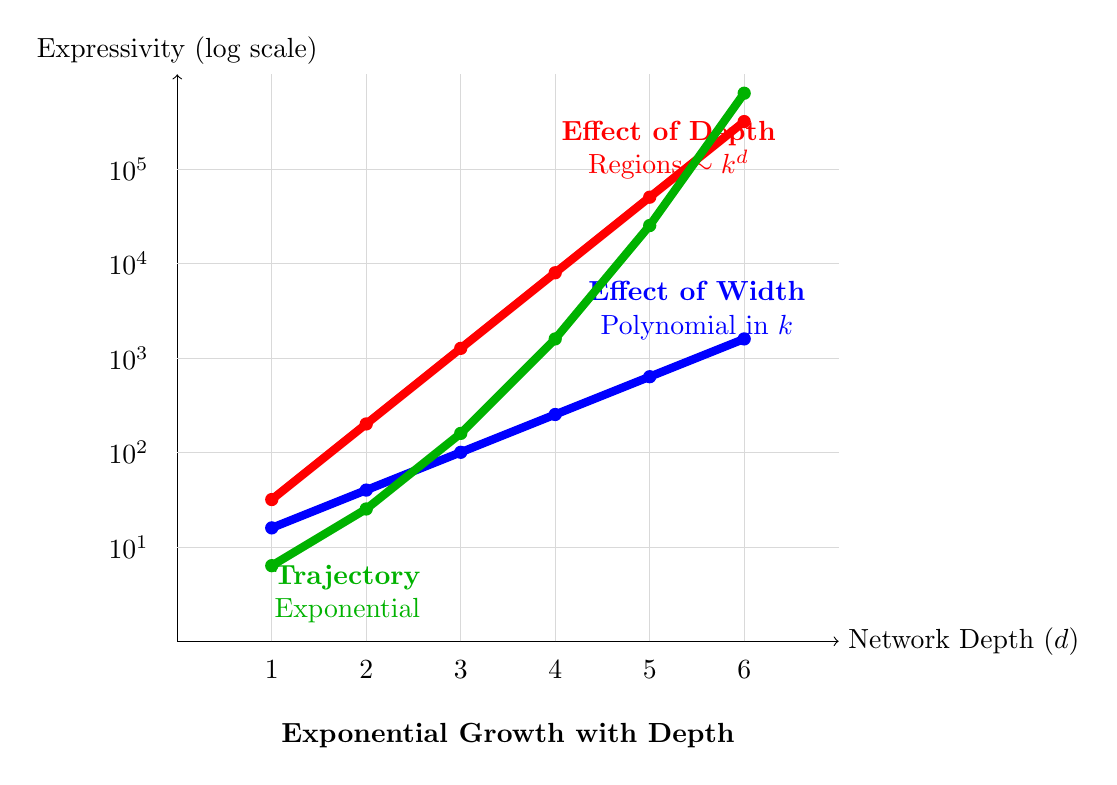
\begin{tikzpicture}[scale=1.2]
    % Main plot
    \draw[->] (0,0) -- (7,0) node[right] {Network Depth ($d$)};
    \draw[->] (0,0) -- (0,6) node[above] {Expressivity (log scale)};
    
    % Grid
    \foreach \x in {1,2,3,4,5,6} {
        \draw[very thin, gray!30] (\x, 0) -- (\x, 6);
    }
    \foreach \y in {1,2,3,4,5} {
        \draw[very thin, gray!30] (0, \y) -- (7, \y);
    }
    
    % Exponential curve for number of regions with depth
    \draw[red, line width=3pt] plot coordinates {(1,1.5) (2,2.3) (3,3.1) (4,3.9) (5,4.7) (6,5.5)};
    \foreach \x/\y in {1/1.5, 2/2.3, 3/3.1, 4/3.9, 5/4.7, 6/5.5} {
        \fill[red] (\x, \y) circle (2pt);
    }
    \node[red, align=center] at (5.2, 5.2) {\textbf{Effect of Depth}\\Regions $\sim k^{d}$};
    
    % Polynomial curve for width effect
    \draw[blue, line width=3pt] plot coordinates {(1,1.2) (2,1.6) (3,2.0) (4,2.4) (5,2.8) (6,3.2)};
    \foreach \x/\y in {1/1.2, 2/1.6, 3/2.0, 4/2.4, 5/2.8, 6/3.2} {
        \fill[blue] (\x, \y) circle (2pt);
    }
    \node[blue, align=center] at (5.5, 3.5) {\textbf{Effect of Width}\\Polynomial in $k$};

    % Trajectory length (exponential)
    \draw[green!70!black, line width=3pt] plot coordinates {(1,0.8) (2,1.4) (3,2.2) (4,3.2) (5,4.4) (6,5.8)};
    \foreach \x/\y in {1/0.8, 2/1.4, 3/2.2, 4/3.2, 5/4.4, 6/5.8} {
        \fill[green!70!black] (\x, \y) circle (2pt);
    }
    \node[green!70!black, align=center] at (1.8, 0.5) {\textbf{Trajectory}\\Exponential};
    
    % Y-axis labels (log scale)
    \node[left] at (-0.2, 1) {$10^1$}; 
    \node[left] at (-0.2, 2) {$10^2$}; 
    \node[left] at (-0.2, 3) {$10^3$};
    \node[left] at (-0.2, 4) {$10^4$}; 
    \node[left] at (-0.2, 5) {$10^5$};
    
    % X-axis labels
    \foreach \x in {1,2,3,4,5,6} {
        \node[below] at (\x, -0.1) {\x};
    }
    
    \node at (3.5, -1) {\textbf{Exponential Growth with Depth}};
\end{tikzpicture}
\caption{The expressivity of neural networks grows exponentially with depth but only polynomially with width. This explains why deep networks are so much more powerful than wide shallow networks.}
\label{fig:depth_vs_width}
\end{figure}


\section{The Hierarchical Feature Learning Story (A Cautionary Tale)}

\subsection{The Idealized Vision}
The geometric picture of compounding complexity leads to a powerful and intuitive story about what deep networks do: they learn a \textbf{hierarchy of features}. The idea is that a complex problem, like identifying a face in an image, can be broken down into simpler sub-problems.

\begin{figure}[h!]
\centering
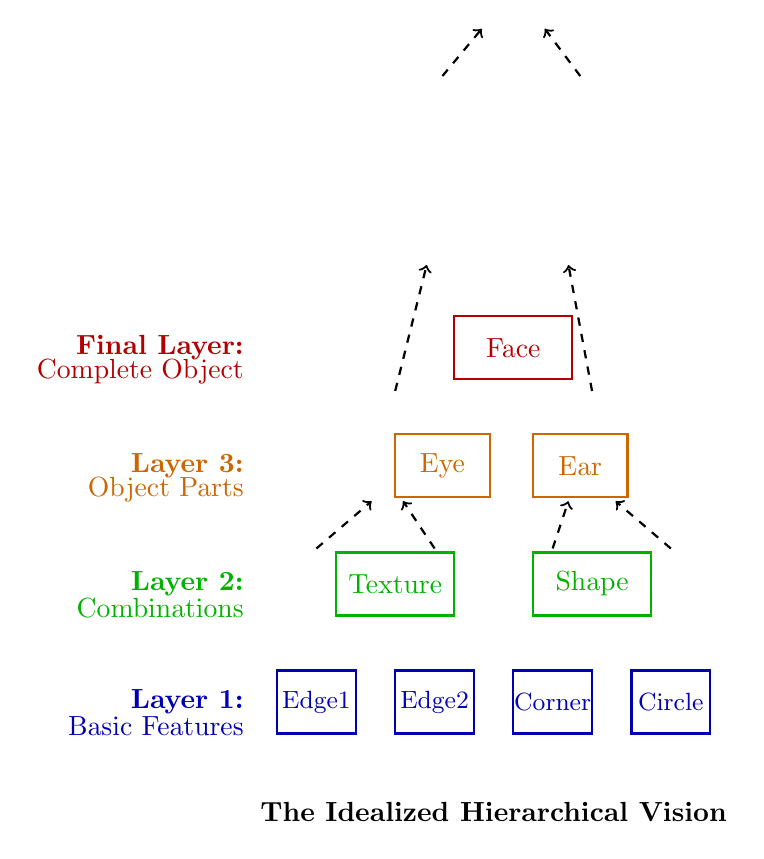
\begin{tikzpicture}[scale=1.0]
    % Layer 1: Edge detectors
    \begin{scope}[yshift=0cm]
        \foreach \i/\label in {0/Edge1, 1.5/Edge2, 3/Corner, 4.5/Circle} {
            \draw[thick, blue!70!black] (\i,0) rectangle ++(1,0.8);
            \node[blue!70!black, font=\small] at (\i+0.5, 0.4) {\label};
        }
        \node[blue!70!black, left] at (-0.3, 0.4) {\textbf{Layer 1:}};
        \node[blue!70!black, left] at (-0.3, 0.1) {Basic Features};
    \end{scope}
    
    % Layer 2: Combinations
    \begin{scope}[yshift=1.5cm]
        \foreach \i/\feature in {0.75/Texture, 3.25/Shape} {
            \draw[thick, green!70!black] (\i,0) rectangle ++(1.5,0.8);
            \node[green!70!black] at (\i+0.75, 0.4) {\feature};
        }
        \node[green!70!black, left] at (-0.3, 0.4) {\textbf{Layer 2:}};
        \node[green!70!black, left] at (-0.3, 0.1) {Combinations};
        
        % Arrows showing combination - but make them dashed to indicate this is idealized
        \draw[->, thick, dashed] (0.5, 0.85) -- (1.2, 1.45);
        \draw[->, thick, dashed] (2, 0.85) -- (1.6, 1.45);
        \draw[->, thick, dashed] (3.5, 0.85) -- (3.7, 1.45);
        \draw[->, thick, dashed] (5, 0.85) -- (4.3, 1.45);
    \end{scope}
    
    % Layer 3: Object parts
    \begin{scope}[yshift=3cm]
        \foreach \i/\feature in {1.5/Eye, 3.25/Ear} {
            \draw[thick, orange!80!black] (\i,0) rectangle ++(1.2,0.8);
            \node[orange!80!black] at (\i+0.6, 0.4) {\feature};
        }
        \node[orange!80!black, left] at (-0.3, 0.4) {\textbf{Layer 3:}};
        \node[orange!80!black, left] at (-0.3, 0.1) {Object Parts};
        
        % Arrows from layer 2 - dashed
        \draw[->, thick, dashed] (1.5, 1.35) -- (1.9, 2.95);
        \draw[->, thick, dashed] (4, 1.35) -- (3.7, 2.95);
    \end{scope}
    
    % Layer 4: Full object
    \begin{scope}[yshift=4.5cm]
        \draw[thick, red!70!black] (2.25,0) rectangle ++(1.5,0.8);
        \node[red!70!black] at (3, 0.4) {Face};
        \node[red!70!black, left] at (-0.3, 0.4) {\textbf{Final Layer:}};
        \node[red!70!black, left] at (-0.3, 0.1) {Complete Object};
        
        % Arrows from layer 3 - dashed
        \draw[->, thick, dashed] (2.1, 3.85) -- (2.6, 4.45);
        \draw[->, thick, dashed] (3.85, 3.85) -- (3.4, 4.45);
    \end{scope}
    
    \node at (2.75, -1) {\textbf{The Idealized Hierarchical Vision}};
\end{tikzpicture}
\caption{The conceptual goal of deep learning is to learn a hierarchy of features. However, standard feedforward networks lack the necessary inductive bias to learn this structure effectively for spatial data, a challenge that motivates specialized architectures like CNNs.}
\label{fig:hierarchical_features}
\end{figure}

\begin{itemize}
    \item \textbf{Early Layers} might learn to detect simple patterns like edges and corners.
    \item \textbf{Middle Layers} could learn to combine these simple features into more complex concepts like eyes, noses, or ears.
    \item \textbf{Final Layers} might then assemble these parts to identify a complete face.
\end{itemize}

\subsection{The Challenge with Fully-Connected Networks}
While this is a beautiful conceptual model, it is \textbf{not} what standard deep feedforward networks (also known as Multilayer Perceptrons, or MLPs) typically do when applied to raw data like images. The idealized vision runs into a critical practical problem: a lack of appropriate \textit{inductive bias}.

In a standard feedforward network, every neuron in a layer is connected to \textit{every} neuron in the previous layer. When the input is an image, this means a single neuron in the first hidden layer looks at all pixels simultaneously. It has no built-in knowledge of spatial locality; it does not know that pixel (10, 10) is closer to (10, 11) than it is to (500, 500).

\subsection{The Reality: A Look Ahead to CNNs}
Because they lack a spatial bias, MLPs often learn ``features'' that are not easily interpretable by humans as local patterns like edges. Instead, they learn complex, non-local combinations of pixels across the entire image that happen to minimize the loss function. This struggle to learn robust, generalizable visual features was a major bottleneck in the history of AI and contributed to challenges in image detection for early neural network models.

This exact problem motivated the development of specialized architectures. \textbf{Convolutional Neural Networks (CNNs)}, which we will discuss in a future lecture, are designed with specific inductive biases (local connectivity, weight sharing) that force them to learn in a spatially structured, hierarchical way. It is within these specialized architectures that the beautiful story of hierarchical feature learning truly becomes a reality.

\section{Practical Implications}
This geometric view has profound practical implications:
\begin{enumerate}
    \item \textbf{Architecture Design}: We understand why deep networks are more efficient than shallow ones—they achieve exponential expressivity with fewer parameters. However, for spatial data like images, we need architectures with appropriate inductive biases.
    
    \item \textbf{Parameter Sensitivity}: Lower layers create the fundamental partitions. Small changes in their weights can cause exponentially amplified changes in the network's output.
    
    \item \textbf{Training Dynamics}: The exponential growth of trajectory length helps explain why training deep networks can be unstable and why techniques like batch normalization, which helps control this growth, are so effective.
    
    \item \textbf{The Importance of Inductive Bias}: Standard feedforward networks, while theoretically powerful, often struggle with structured data like images because they lack built-in assumptions about the problem structure. This motivates specialized architectures.
\end{enumerate}

This perspective transforms neural networks from mysterious black boxes into interpretable geometric machines that systematically partition space to solve complex problems. However, it also reveals why the choice of architecture—and the inductive biases it embeds—is crucial for success on real-world tasks.

\end{document}